\documentclass[11pt]{article}

\usepackage[T1]{fontenc}
\usepackage[utf8]{inputenc}
\usepackage{lmodern}
\usepackage[a4paper,margin=29mm]{geometry}
\usepackage{amsmath,amssymb}
\usepackage{booktabs,longtable,array,tabularx}
\usepackage{enumitem}
\usepackage{graphicx}
\usepackage{microtype}
\usepackage{xcolor}
\usepackage{hyperref}
\usepackage[capitalise,noabbrev]{cleveref}
\hypersetup{hidelinks}

\newcommand{\systemname}[1]{\textsc{#1}}
\newcommand{\evidence}[1]{\textit{#1}}
\newcommand{\filepath}[1]{\path{#1}}
\newcommand{\excerptlink}[2]{\hyperref[ex:#1]{Supplementary Excerpt~#2}}

\newcommand{\CatalogueRows}{117}
\newcommand{\PositiveRows}{94}
\newcommand{\NegativeRows}{23}
\newcommand{\DirectCertificateRows}{20}
\newcommand{\PureChordalRows}{19}
\newcommand{\FailedRoutes}{65}
\newcommand{\ProofNotes}{57}
\newcommand{\CorrespondenceNotes}{33}
\newcommand{\TypedPrompts}{86}
\newcommand{\GoalObjectives}{10}
\newcommand{\WorkstationCodexTurns}{107}
\newcommand{\WorkstationCodexTokens}{1,912,053,938}
\newcommand{\WorkstationCodexCached}{1,868,302,720}
\newcommand{\SecondPrimaryTurns}{40}
\newcommand{\SecondCodexTokens}{669,491,502}
\newcommand{\UltraTurns}{11}
\newcommand{\UltraHours}{4.16}
\newcommand{\ClaudeInputTokens}{283,520,656}
\newcommand{\ClaudeOutputTokens}{1,333,543}
\newcommand{\ChatGPTCampaignConversations}{9}
\newcommand{\ChatGPTSatelliteConversations}{7}
\newcommand{\ApprovalReviews}{45}
\newcommand{\CampaignCommits}{40}
\newcommand{\ClaudeTrailerCommits}{16}
\newcommand{\BoundedRuns}{20}
\newcommand{\BoundedHours}{11.69}
\newcommand{\BoundedPeakGiB}{11.91}
\newcommand{\AtlasFortyThreeModules}{1,097}
\newcommand{\AtlasFortyThreeHours}{6.0}
\newcommand{\AtlasFortyThreePeakGiB}{15.4}


\title{Codex, Claude Code, and ChatGPT Pro in a Formalized\\
Graphon Classification: An Observational Case Study}
\author{Author names to be confirmed\thanks{The author list and affiliations will be inserted after confirmation.}}
\date{Draft of \today}

\begin{document}
\maketitle

\begin{abstract}
We reconstruct a six-week AI-assisted research campaign that classified a
chromatic-polynomial graphon inequality for all $117$ relevant graphs on at
most six vertices.  The resulting companion mathematics paper reports $94$
positive and $23$ negative rows, with all rows represented by Lean theorems.
The present article asks how ChatGPT Pro, Codex, and Claude Code moved from
proof search to checkable artifacts.  Its evidence consists of surviving
prompts and responses, session indexes, git history, mathematical notes,
exact certificates, Lean sources, failure ledgers, and retained sequential
build measurements.  Five contrasts are supported.  First, Codex did not
merely translate the Atlas~43 proof: it found a shared-edge semantic error,
repaired the probabilistic interpretation, reported the repair, and withheld
verified status pending the remaining exact checks.  Second, memory and time
constraints changed proof objects: large certificates were decomposed or
compressed, and Claude Code replaced an infeasible stronger route for
Atlas~127 by a smaller row-level certificate.  Third, formalization often
narrowed a general informal theorem to the exact proposition needed for one
classification row.  Fourth, Codex used several proof families in a recurring
order before turning to general rooted sum-of-squares certificates.  Fifth,
the successful long Codex run occurred in a particular operating regime---a
continuous, tightly specified task with reusable exact-certificate tooling---
whereas the available high, xhigh, and ultra sessions do not isolate a causal
effect of reasoning effort.  Because the campaign was not controlled and
some source material is missing, we conclude with a prespecified clean-rerun
protocol rather than a model-ranking claim.
\end{abstract}

\section{Introduction}

Language-model theorem proving is often evaluated as a collection of short,
independent theorem attempts.  Systems such as GPT-f, LeanDojo, and Baldur
measure formal proof generation or repair under controlled benchmark
conditions~\cite{PoluSutskever2020,YangEtAl2023,FirstEtAl2023}.  Other systems
combine learned proposals with symbolic evaluation to search for new
mathematical constructions~\cite{RomeraParedesEtAl2024,TrinhEtAl2024}.  The
campaign studied here has a different shape.  It lasted from 13~August to
23~September 2026, used three commercial interfaces over many sessions, and
ended in a repository containing mathematical notes, exact rational
certificates, Lean sources, and verification scripts for a finite research
classification.

The mathematical question is the following.  For a finite graph $H$ and a
graphon $W$ of edge density $p$, define
\begin{equation}
 \Phi_H(p)=(1-p)^{v(H)}\chi_H\!\left(\frac{1}{1-p}\right).
 \label{eq:target}
\end{equation}
For each non-bipartite graph $H$ on at most six vertices, excluding isolated
vertices and isolated-edge components, the project asked whether
\begin{equation}
 t(H,W)\geq \Phi_H(p)
 \quad\text{whenever}\quad
 p\geq 1-\frac{1}{\chi(H)-1}.
 \label{eq:inequality}
\end{equation}
There are $117$ isomorphism classes in scope.  The companion mathematics
paper proves that $94$ satisfy \eqref{eq:inequality} and $23$ do
not~\cite{CompanionMath2026}.  This article does not repeat those proofs.  It
studies the route by which the proof artifacts were created and checked.

The headline claim is not that verification is useful.  Rather, the surviving
materials expose several non-equivalent transitions that the word
``verification'' can hide: testing the semantics of an informal identity,
checking exact coefficient equalities, translating a certificate into Lean,
auditing theorem status, and compiling a large source tree within a stated
resource envelope.  Different transitions caught different problems.  They
also fed back into the mathematics by changing which theorem or certificate
was used.

This is an observational case study.  ChatGPT Pro, Codex, and Claude Code were
not assigned matched tasks under fixed conditions.  Model versions, reasoning
effort, prompt form, repository state, session continuity, and elapsed time
changed together.  The human author also chose the allocation of work and
the acceptable proof standard.  Consequently, the paper supports claims
about what happened within this campaign, but not causal comparisons among
vendors, interfaces, or effort settings.

The contributions are:
\begin{enumerate}[leftmargin=2em]
 \item an evidence-linked reconstruction of a long mathematical campaign,
 with exact quotations separated into a chronological supplement;
 \item five findings based on before--after or cross-stage contrasts rather
 than on the mere existence of a workflow component;
 \item an analysis of proof-object size as part of mathematical proof search,
 illustrated by Atlas~43 and Atlas~127;
 \item a separation between theorem discovery, row closure, exact checking,
 Lean formalization, and fresh compilation; and
 \item a protocol for a future clean rerun that could test hypotheses which
 the historical campaign alone cannot settle.
\end{enumerate}

\section{Case and participants}
\label{sec:case}

\subsection{Mathematical endpoint}

The campaign ended with a complete $94/23$ classification.  Positive rows
were covered by analytic families, closure arguments, row-specific
inequalities, or exact rooted sum-of-squares certificates.  Every negative
row received an exact rational step-graphon witness.  The repository contains
$117$ Lean example modules whose final status fields are
\texttt{.verified}; a source scan finds no \texttt{sorry} in those modules.
The author additionally reports checking a successful full build on another
device.  The directory for that build and its exact start and end times are
not present in this checkout, so this article distinguishes the author
statement from the retained row-level build measurements.

The companion mathematics paper is the authority for the theorem, proof
families, counterexamples, and formal statements.  Here the $117$ rows are
units whose status changes over time: \emph{claimed resolved} when a positive
proof or negative witness was asserted, and \emph{Lean-marked verified} when
the repository status said that a Lean theorem had been completed.  The
second label follows historical source state; it does not itself certify that
a fresh full build had already occurred.

\subsection{Systems and assigned roles}

\Cref{tab:systems} summarizes how the three interfaces appear in the surviving
materials.  These roles were largely assigned by the human author.  Their
division is therefore provenance, not a finding that the systems
spontaneously specialized.

\begin{table}[t]
\centering
\small
\caption{AI systems in the campaign.  Model identifiers are stated only where
the surviving session source supplies them.}
\label{tab:systems}
\begin{tabularx}{\textwidth}{p{2.7cm} X X}
\toprule
interface & observed use & surviving evidence\\
\midrule
ChatGPT Pro & conceptual theorem search, informal derivations, and proposed
proof directions & nine campaign and seven satellite conversations in the
export; files and some reasoning context are absent\\
Codex & repository-wide classification, computational searches, proof notes,
certificate infrastructure, Lean code, and status maintenance & two device
indexes, including \WorkstationCodexTurns{} workstation turns and
\SecondPrimaryTurns{} second-device primary turns; important sessions identify
\texttt{gpt-5.6-sol} and their effort settings\\
Claude Code & later audit, certificate compaction, source compilation, and
completion of the final rows & retained Claude Code sessions, including
\texttt{claude-fable-5-1} and \texttt{claude-opus-5}, plus generated source and
build summaries\\
\bottomrule
\end{tabularx}
\end{table}

The author states that neither human collaborator wrote proof text,
certificate files, scripts, or Lean code in this campaign.  They supplied
prompts and transferred outputs among interfaces and machines.  Surviving
patch-level sessions support that statement where such sessions remain, but
deleted Claude Code conversations and pasted outputs prevent an archive-only
proof of a universal negative.  We therefore present it as an author
declaration corroborated by the available traces.

\section{Materials and reconstruction method}
\label{sec:method}

\subsection{Corpus}

The reconstruction uses seven kinds of material:
\begin{enumerate}[leftmargin=2em]
 \item machine-readable Codex and Claude Code session indexes from two
 devices, with turn times, prompts, final responses, token counters, and file
 references;
 \item a ChatGPT export extract and a manually reconstructed prompt appendix;
 \item git commits, trailers, and source timestamps;
 \item the live $117$-row catalogue and the numbered failed-route ledger;
 \item mathematical notes and note-to-Lean correspondence sections;
 \item exact certificate and counterexample checkers; and
 \item retained per-row and Atlas~43 sequential-build summaries.
\end{enumerate}

We classify a statement as \evidence{logged} when it occurs in a surviving
prompt or response, \evidence{source-level} when it is directly supported by
the mathematical or Lean files, \evidence{computed} when a supplied script
reconstructs it, \evidence{author-attested} when it depends on the author's
recollection, and \evidence{inferred} when it is reconstructed from indirect
agreement among sources.  The main findings below rely primarily on logged,
source-level, and computed support.  Inferences are labelled.

The campaign boundary starts with the six-vertex census on 13~August and ends
with the completion of Atlas~127 on 23~September.  June--July ChatGPT work and
an earlier, independent odd-cycle project are excluded.  This matters because
the odd-cycle theorem used in the classification was proved by a different
route.

\subsection{Counting rules}

The reconstruction script counts typed prompts, goal-interface objectives,
turns, source transitions, failed routes, commits, and retained build
summaries.  Provider token counters are retained separately.  Codex processed
tokens include cache traffic; Claude Code exposes a different decomposition;
and a Lean build can occur inside a timed model turn.  We therefore neither
add all token counters nor sum turn durations and compilation time into one
cost.

Figure~\ref{fig:completion} uses cumulative active Codex and Claude Code turn
time from surviving logs as an effort proxy.  Parallel turns are additive.
The horizontal axis excludes human time, ChatGPT web activity,
retention-deleted August Claude Code sessions, and stand-alone builds outside
a logged turn.  The plot is useful for chronology, not for productivity
estimation.  It also exposes the long interval between claimed resolution and
formal status for many rows.  The first firm intermediate formalization
checkpoint is Claude Code's 18 August working note, which counted 84
Lean-marked rows.  A completed rebuild established 94 rows before the later
bulk commit; the commit itself is therefore not treated as the verification
event.

\begin{figure}[t]
\centering
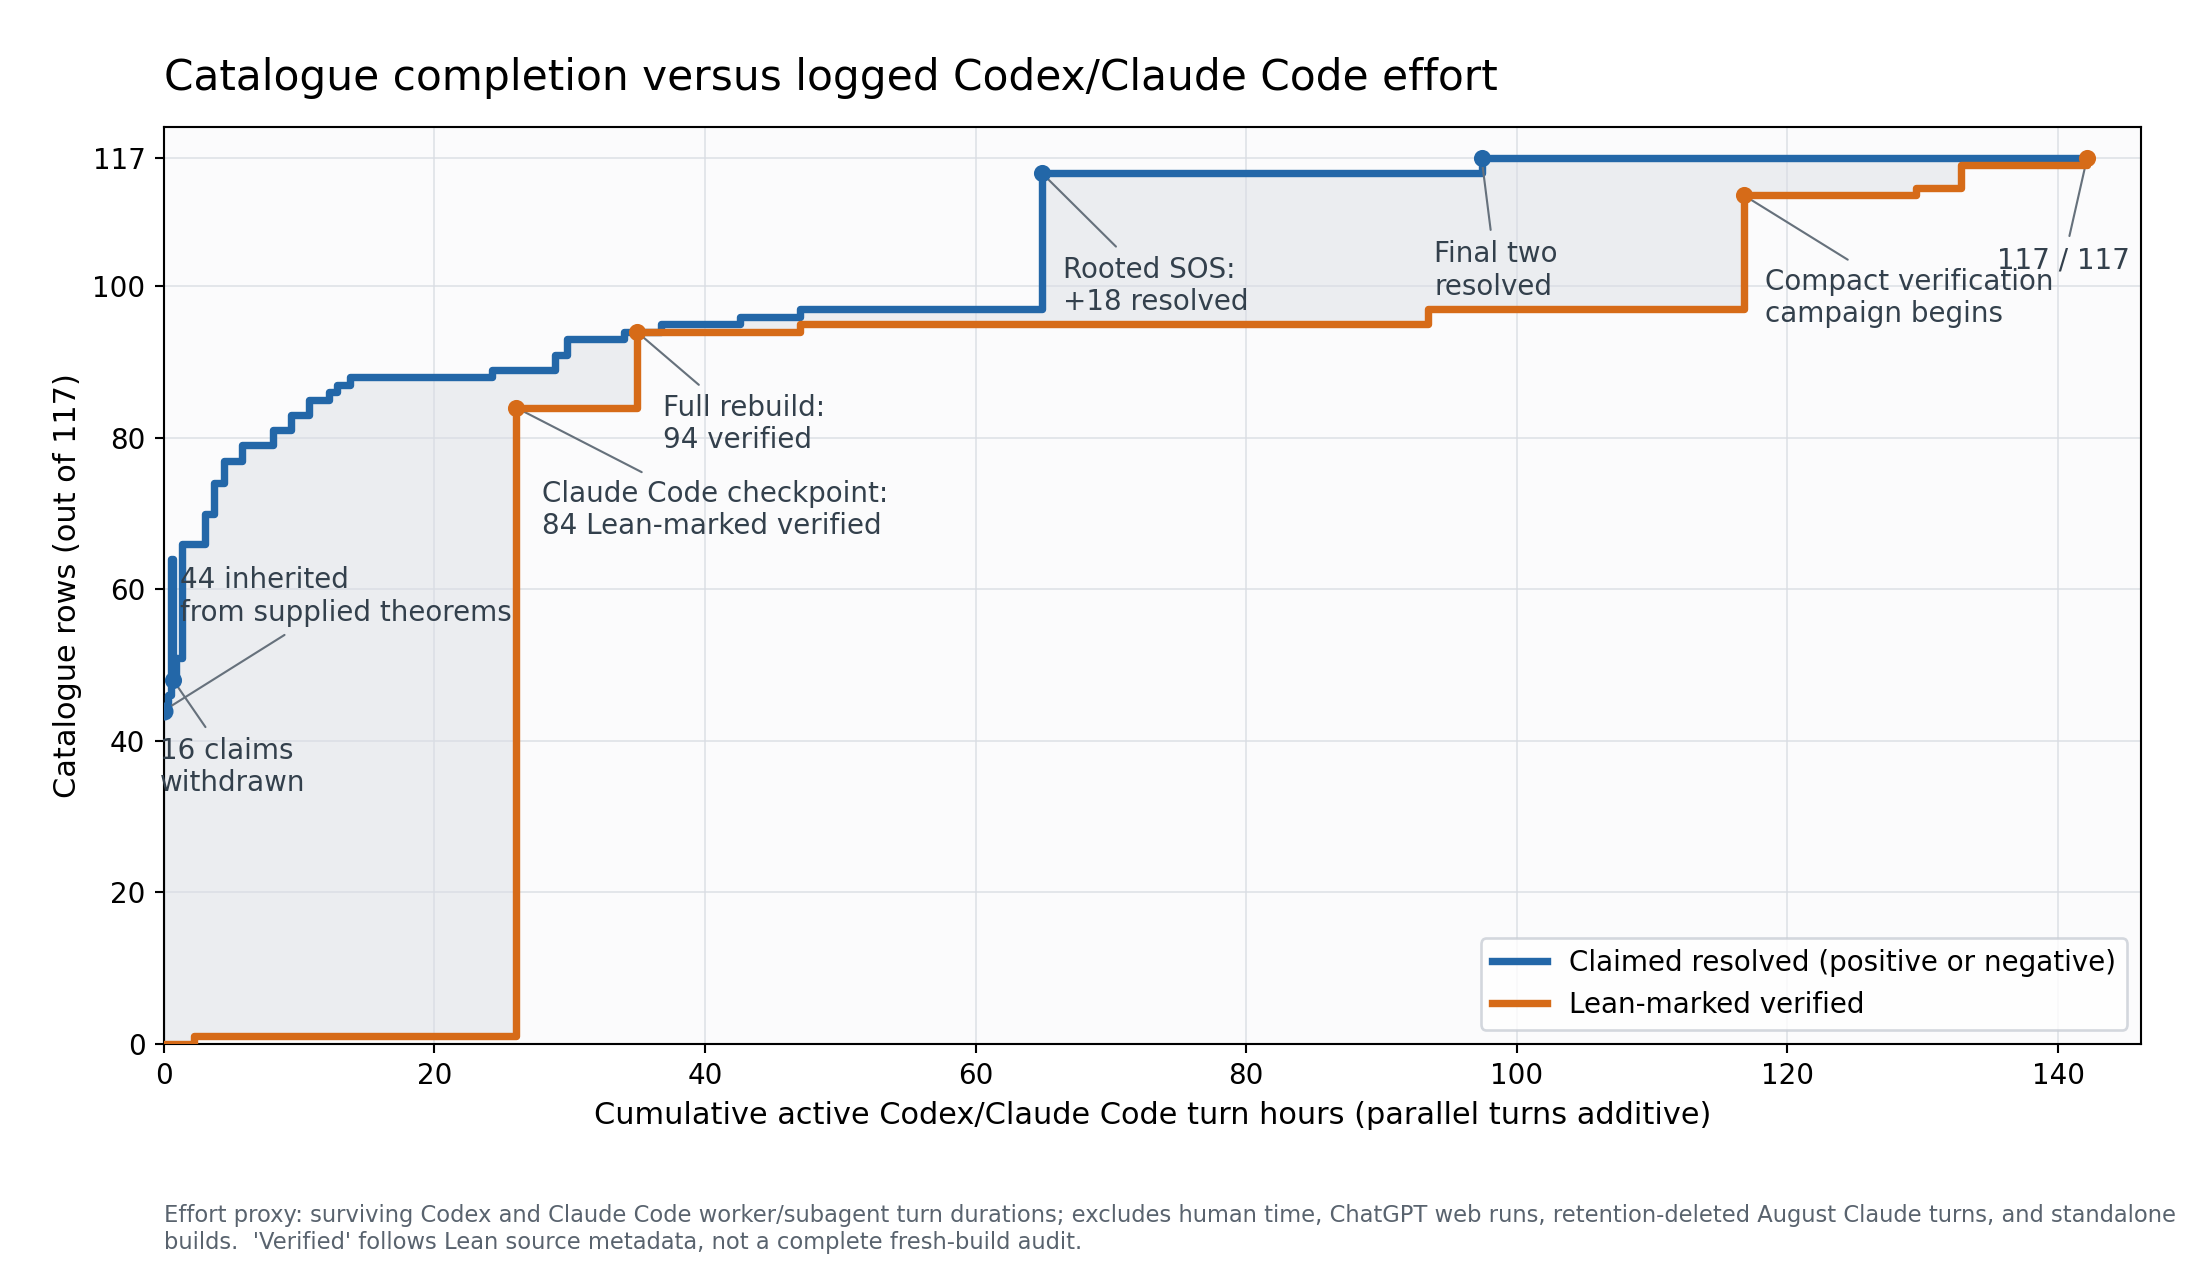
\includegraphics[width=\textwidth]{../completion_vs_effort.png}
\caption{Catalogue progress against an incomplete, non-additive effort proxy.
The blue curve follows claimed mathematical resolution; the orange curve
follows historical Lean status.  Neither curve should be interpreted as a
controlled learning curve.}
\label{fig:completion}
\end{figure}

\subsection{Selection of conversation evidence}

The main text paraphrases operational exchanges in professional language.
Supplementary Appendix~\ref{app:excerpts} preserves selected source text with
a stable excerpt label, date, speaker, model where known, session identifier,
turn, and prompt identifier.  An exchange is included only if it changed
mathematical correctness, proof status, verification scope, resource policy,
or research direction.  This selection rule avoids treating candid wording
as spectacle while allowing the reader to inspect the claims made here.

\section{Findings}
\label{sec:findings}

\subsection{A formalization request triggered a reported semantic repair}
\label{sec:repair}

Atlas~43 entered the formalization stage with a rooted sum-of-squares
identity.  In a 25~August Codex turn, the human author asked for Lean
implementation of the unformalized proofs.  Codex tested the proposed rooted
semantics on the constant graphon $W\equiv 1/2$ and found that the two sides
did not agree.  The cause was repeated use of the same labelled edge: the
informal identity treated that shared Bernoulli edge as if its conditional
means multiplied independently, replacing $W$ by $W^2$.

Codex changed the semantics so repeated appearances referred to one shared
Bernoulli edge variable.  The Gram matrices and the $91$ exact coefficient
equalities remained applicable.  Thus, this was a repair to the bridge from
the certificate algebra to graphon density, not a replacement certificate.
Codex prominently reported the error and its repair, and left Atlas~43 at
\texttt{believed} until the remaining coefficient chain had been imported and
checked; see \excerptlink{B12}{B.1.2}.  It did not ask the human author to
supply a revised proof.

The observable behavior supports a limited explanation.  Codex treated the
problem as locally repairable because the numerical and rational certificate
components survived the semantic correction.  Private reasoning is not
available, so the paper does not claim access to why Codex chose repair over
requesting a new proof.  Nor did the same $W^2=W$ mistake recur independently
row by row.  It was one common-framework error.  Other mistakes occurred---a
reversed-Jensen draft, rejected intermediate lemmas, stale status fields---but
they were different failures.

This episode is more specific than the truism that checking helps.  Three
states diverged: the finite Gram identity could be right, its probabilistic
interpretation could be wrong, and the row could remain short of an end-to-end
Lean check.  The Codex response separated those states rather than reporting
an undifferentiated success.

\subsection{Resource constraints changed the proof object}
\label{sec:resources}

The project imposed a practical per-row envelope of roughly one hour,
$16$~GiB, and about $100$ generated files for the compact-certificate phase.
This was not merely a scheduling choice.  It selected among mathematically
equivalent or sufficient representations.

Atlas~43 provides the first example.  A parallel Lean invocation spawned
eight workers at about $13.5$~GB each and exhausted machine memory.  Claude
Fable explicitly attributed the crash to its bare parallel build and noted
that the existing verification driver was sequential
(\excerptlink{B22}{B.2.2}).  Claude Fable then compiled all
\AtlasFortyThreeModules{} modules sequentially in \AtlasFortyThreeHours{}
hours, with a \AtlasFortyThreePeakGiB{}~GiB peak
(\excerptlink{B23}{B.2.3}).  Sequential checking made that already-decomposed
proof feasible, but did not make it compact.

Atlas~127 shows a stronger mathematical change.  Claude Opus measured a
ground-$8$ route intended to formalize a smoothed-Goodman theorem.  An
order-$272$ source component used $16.20$~GiB before reaching its proof checks
and was killed under the cap.  Claude Opus projected $800$--$1{,}200$ files
and $25$--$40$ sequential hours, and explained why splitting source tables
would not split the single large positive-semidefinite kernel computation
(\excerptlink{B32}{B.3.2}).

After the author rejected a day-long compilation for one small theorem,
Claude Opus weakened the target from the stronger general theorem to the
Atlas~127 row itself.  A direct ground-$6$ certificate passed the first
numerical gate (\excerptlink{B34}{B.3.4}).  A single interval still placed the
Gram point on a singular face, but splitting at $p=2/3$ produced two
full-rank pieces that rationalized exactly
(\excerptlink{B35}{B.3.5}).  The resulting row used $97$ files, $2617.5$
seconds, and $11.90$~GiB, completing the $117$-row Lean status
(\excerptlink{B36}{B.3.6}).

These episodes identify three distinct responses to size:
\begin{enumerate}[leftmargin=2em]
 \item \emph{decompose} the check and execute components sequentially;
 \item \emph{compress} a numerical search result into sparse rational
 certificate components; and
 \item \emph{replace} a stronger theorem by a smaller sufficient statement,
 then split its parameter interval to move into the interior of the exact
 cone.
\end{enumerate}
The choice was not made by the human author alone.  The author set the
envelope and rejected the oversized route; Claude Opus measured the failure,
identified the row-level alternative, diagnosed the singular single interval,
and produced the split certificate.  The resulting technical lesson is not
that a small certificate is always preferable.  It is that verifiability adds
a second optimization problem: one must search for a proof object whose exact
checking computation fits the available environment.

\subsection{Formalization narrowed and reorganized the mathematics}
\label{sec:refactoring}

Several informal notes stated general theorems whose full formalization was
unnecessary for the finite classification.  The Lean development often kept
only the specialization needed for one row.  This changed dependencies and,
in some cases, exposed a shorter proof.

For Atlas~153, 171, 174, and 188, a target-sign observation removed
self-amalgamation and Fisher-profile machinery from the route ultimately
checked.  Atlas~160 and 178 were reduced to smaller polynomial obligations.
On the negative side, explicit tensor-product step graphons replaced an
asymptotic theorem by finite rational evaluations.  Atlas~127 likewise ended
with the direct ground-$6$ certificate rather than a formal proof of the
stronger smoothed-Goodman statement.

This distinction must be stated precisely.  The project does not claim that
Lean contains every general theorem discussed in the mathematical notes.  It
claims that the Lean sources prove the $117$ row propositions, with reusable
formal machinery for several families and row-specific endpoints elsewhere.
The behavioral contrast is between informal theorem construction, which often
favored conceptual scope, and formal row closure, which favored the weakest
exact statement sufficient for the classification.

\subsection{Codex used diverse methods in a recurring search order}
\label{sec:breadth}

The evidence does not support a claim that Codex had one fixed preferred proof
method.  Across the surviving sessions, it used tensor products of Tur\'an
graphons for negative rows; whiskering, self-amalgamation, cones, normalized
links, and clique-tree arguments for positive families; supporting-plane,
projection, and polynomial arguments for individual rows; and rooted
sum-of-squares certificates for the remaining residue.

There was nevertheless a recurring order.  Codex first searched for reusable
families and closure principles, next developed row-specific analytic
reductions, and finally built general rooted-certificate infrastructure for
the unresolved cases.  The failure ledger grew to \FailedRoutes{} numbered
routes and frequently distinguished a failed intermediate lemma from a
counterexample to the target theorem.  This hierarchy explains why the final
long certificate turn was not simply an isolated burst of computation: it
operated after broad families and cheaper special arguments had reduced the
residue to twenty rows.

In the 25~August xhigh turn, the author asked Codex to resolve all twenty
remaining cases, favoring positive proofs unless there was a strong negative
indication and allowing computational exact certificates.  Over about
$10.5$ hours, Codex built reusable certificate machinery and closed eighteen
rows.  It left Atlas~130 and 203 partial and described a final $42$-minute
solver failure as yielding no certificate or mathematical conclusion; see
\excerptlink{B42}{B.4.2}.  The combination of methodological breadth and
explicitly limited failure reporting is stronger evidence than a bare count
of attempted methods.

\subsection{The evidence indicates an operating regime, not a winning effort tier}
\label{sec:effort}

The productive Codex turn used xhigh reasoning effort, while eleven live ultra
turns on the second device totalled $4.16$ hours and closed no row.  The only
high Codex proving turn in the relevant comparison was a $28$-minute failed
audit.  A simple slogan that higher reasoning effort is worse would be
unsupported.  The sessions differ in task, duration, context, continuity,
model state, and available tooling.

What can be said is narrower and more useful.  Closure occurred in a regime
combining four features: a long uninterrupted turn, a sharply stated
finite-row objective, permission to build exact computational machinery, and
a residue already prepared by previous analytic work.  The xhigh label is one
part of that configuration.  The ultra attempts were shorter and fragmented;
the high attempt was both short and aimed at a different audit problem.  Thus,
the history motivates a hypothesis that there is a suitable allocation of
continuity, tool-building effort, and task scope.  It does not estimate the
independent effect of a reasoning-effort setting.

\section{What the quantitative traces do and do not show}
\label{sec:quantitative}

\begin{table}[t]
\centering
\small
\caption{Observable campaign quantities.  Token counters retain each provider's semantics and are not added across providers.}
\label{tab:campaign-quantities}
\begin{tabular}{p{5.5cm} r p{6.0cm}}
\toprule
quantity & value & definition\\
\midrule
Human prompts in the workstation appendix & 86 & typed prompts to Codex or Claude Code\\
Codex goal objectives & 10 & goal-interface objectives\\
Workstation Codex worker turns & 107 & all extracted Codex worker turns\\
Second-device primary live turns & 40 & non-replayed primary Codex turns\\
Workstation Codex processed tokens & 1,912,053,938 & provider counter; includes cache traffic\\
Second-device Codex processed tokens & 669,491,502 & provider counter; primary threads\\
Claude Code input tokens & 283,520,656 & input plus cache read and cache creation\\
Claude Code output tokens & 1,333,543 & surviving workstation sessions\\
ChatGPT Pro conversations & 16 & campaign plus satellite conversations\\
Automatic approval reviews & 45 & 29 workstation plus 16 second-device requests\\
Numbered failed routes & 65 & entries in the failure ledger\\
Bounded sequential row builds & 20 & 11.69 h combined; peak 11.91 GiB\\
Atlas 43 sequential chain & 1,097 & 6.0 h; peak 15.4 GiB\\
\bottomrule
\end{tabular}
\end{table}


The largest counters in \Cref{tab:campaign-quantities} are not comparable
measures of mathematical work.  The workstation Codex total includes
\WorkstationCodexCached{} cached input tokens.  The second-device figure uses
the provider's processed-token counter over primary threads.  Claude Code
separates input, cache traffic, and output differently.  Replayed forks can
also repeat large contexts.  These quantities are useful for auditing the
scale of interaction and the danger of treating context replay as fresh
reasoning; they are not prices or additive compute estimates.

The same caution applies to time.  Twenty retained bounded row builds total
\BoundedHours{} hours, with a largest peak of \BoundedPeakGiB{}~GiB, while the
separate Atlas~43 check took \AtlasFortyThreeHours{} hours.  Some compilation
happened inside Claude Code or Codex turns.  Adding model-turn and build time
would double count those intervals.  The surviving sources also omit human
reading time, several deleted sessions, ChatGPT web duration, energy use, and
the unavailable full-build directory.

The author reports a ChatGPT Pro subscription price of KRW~159,000 per month
and Claude Max charges of USD~96.76 on 21~July and USD~110 on 21~September.
These subscriptions covered activity outside the defined campaign.  They are
reported for transparency but are not assigned as a project cost.

\section{Reusable artifacts and epistemic drift}
\label{sec:artifacts}

Two shared files were especially important.  The catalogue maintained one
row per graph with mathematical status, proof reason, witness, and Lean state.
The failed-route ledger preserved negative knowledge, including exact
counterexamples to intermediate lemmas for rows whose target theorem was
eventually positive.  Together they allowed later Codex and Claude Code
sessions to begin from more than a prose handoff.

Their benefit is plausible but not experimentally isolated.  The human author
asked that these files be maintained; the systems did not independently
choose a modular division of labor.  Moreover, the catalogue itself drifted.
Narrative sections and architecture notes lagged behind source changes, a
count module required correction, and Atlas~43 and 196 were marked verified
before the later measured sequential check.  A shared catalogue was therefore
useful working memory and also a boundary at which confidence labels could
get ahead of executable evidence.

The final theorem artifacts are easier to reproduce than their discovery.
Exact rational witnesses, certificate checkers, Lean files, twenty row-build
summaries, and the Atlas~43 compilation summary survive.  Numerical
semidefinite workspaces, some deleted Claude Code transcripts, private model
reasoning, and the full-build directory do not.  A future reader can inspect
many final proof obligations without being able to replay every search choice
that produced them.

\section{A prespecified clean-rerun protocol}
\label{sec:rerun}

The historical material suggests that structured handoffs, exact-certificate
infrastructure, and a resource-aware objective may help close a finite table.
It cannot test that claim.  We propose the following experiment for a future
paper.

\subsection{Snapshot and tasks}

Freeze a repository snapshot immediately before the twenty-row residual
campaign.  Remove later proofs, generated certificates, completion-specific
notes, and commit messages while retaining the common mathematical foundation
available at that date.  Package each residual row with the same statement,
permitted dependencies, and checker interface.  Because rows differ greatly
in difficulty, use the entire twenty-row bundle as the primary task rather
than treating rows as exchangeable independent samples.

\subsection{Matched conditions}

Run at least five independent trials per condition with the same Codex model
version, effort setting, token allowance, wall time, machine class, and base
snapshot.  Compare:
\begin{enumerate}[leftmargin=2em]
 \item a direct instruction to solve the residual rows; and
 \item a structured workflow supplying the catalogue, failed-route format,
 exact-certificate tools, explicit resource envelope, and a requirement to
 separate conjectured, exact-checked, Lean-checked, and fresh-built states.
\end{enumerate}
The human may respond only through a prespecified heartbeat message and may
not contribute new mathematics during a trial.  Any crash-recovery policy and
permission decision must be fixed in advance.

\subsection{Endpoints}

The primary endpoint is the number of rows that pass a fresh Lean build under
the stated envelope.  Secondary endpoints are time to first verified row,
number of exact certificates produced, false positive status transitions,
maximum memory, generated source size, failed routes revisited, and the gap
between claimed proof and fresh compilation.  An independent script should
assign statuses from artifacts rather than from the model's final prose.

A separate factorial experiment is needed to study reasoning effort.  It
should hold the model, snapshot, prompt, tools, wall time, and trial count
fixed while varying only high, xhigh, and ultra.  Without that design, the
current campaign should not be cited as evidence that one effort setting is
better.

\subsection{Threats to the rerun}

Public availability of the completed repository may contaminate later model
versions.  A private isomorphic benchmark or newly generated family would
reduce direct memorization.  Trials may still share provider-side state that
is unavailable to the investigator.  Lean success also favors work already
close to the supplied library.  The protocol therefore tests a workflow on a
bounded formal task; it does not measure mathematical research ability in
general.

\section{Limitations}
\label{sec:limitations}

This study has one campaign, one mathematical domain, and no randomized
assignment.  The human author changed prompts after observing failures, so
interventions are endogenous to progress.  Models and interfaces changed
across sessions.  Several August Claude Code transcripts were removed by
retention, the ChatGPT export omits some context and files, and private model
reasoning is unavailable.  The unavailable full-build directory prevents an
independent reconstruction of that run's environment and timing from this
checkout.

Status labels are historical claims, not substitutes for compilation.  In
particular, the completion curve follows source state and includes the period
when Atlas~43 and 196 were marked verified before the retained sequential
audit.  Token counters have provider-specific meanings, and wall time is
incomplete.  Subscription payments cannot be allocated to this project.

Finally, quotations were selected because they changed correctness, status,
scope, resources, or direction.  They are not a random sample of interaction
quality.  The appendix supplies enough surrounding context to audit the
claims made here, while the full indexes remain necessary for alternative
analyses.

\section{Conclusion}

The campaign shows a progression from broad mathematical search to compact,
machine-checkable row proofs, but its most useful lessons lie in contrasts.
Codex repaired a semantic error while preserving the algebraic certificate;
Claude Code changed an infeasible strong theorem into a feasible row-level
certificate; Lean formalization repeatedly selected smaller sufficient
statements; and Codex moved through several analytic families before building
general exact-certificate machinery.  The successful xhigh run combined
continuity, a finite objective, and reusable tools, so its outcome cannot be
attributed to effort level alone.

For future AI-assisted mathematics, the checkable endpoint should be defined
before the search begins, and proof-object resources should be treated as part
of proof design.  Claims of workflow benefit or model superiority require the
clean matched reruns that this historical campaign did not contain.

\paragraph{AI assistance and conflict disclosure.}
OpenAI Codex (GPT-5) drafted this article from the project sources and wrote
the scripts that regenerate its aggregate counts and curated supplementary
excerpts.  Codex is an OpenAI system, and OpenAI systems are among the subjects
of this case study.  The authors remain responsible for source selection,
interpretation, and the submitted text.

\appendix

\section{Audit definitions and source gaps}
\label{app:audit}

\subsection{Status definitions}

\begin{description}[leftmargin=3.5cm,style=nextline]
 \item[Claimed resolved] A surviving source asserts either a positive proof or
 an exact negative witness for the row.
 \item[Exact-checked] A rational checker verifies the finite certificate or
 witness arithmetic independently of a numerical solver.
 \item[Lean-marked verified] The historical Lean source status is
 \texttt{.verified}; this is the state used by Figure~\ref{fig:completion}.
 \item[Fresh-built] The relevant source was compiled from a specified source
 state in a retained sequential run.
 \item[Full-build attestation] The author reports checking the entire
 development on another device, but the run directory is unavailable here.
\end{description}

\subsection{Known gaps}

The supplied checkout lacks the referenced full-run directory,
\filepath{lean/verification_runs/full-20260923-164651/}; a handoff named
\filepath{HANDOFF_ATLAS_188_171_174_153.md}; and
\filepath{lean/docs/TODO.md}.  A search of the reachable git history did not
recover the latter two paths.  The workstation raw-log backup is absent,
although its extracted index and appendices survive.  The second-device
backup survives.  These gaps chiefly constrain exact discovery provenance
and full-build timing, not the inspectability of the final row sources.

\section{Curated chronological excerpts}
\label{app:excerpts}
The selection rule includes exchanges that changed mathematical correctness, proof status, verification scope, resource policy, or research direction. Wording and typographical errors are retained.  Export-only HTML spacing markers are omitted, and mathematical Unicode glyphs receive equivalent LaTeX typesetting.  Ellipses are not inserted inside an excerpt.

\subsection{The Atlas 43 semantic repair}
\subsubsection*{Excerpt B.1.1}
\phantomsection\label{ex:B11}
\noindent\textit{25 August 2026, 13:21 KST; Codex gpt-5.6-sol, xhigh; session 01a03722, turn 1; prompt A.38; speaker: human author.}
\begin{quote}\small\ttfamily\raggedright
Thank you. There are lots of unverified (unformalised) proofs now. Would you please work on implementing the lean proof? You may find the lean proof existing first to see how the proofs are organised.
\par
\end{quote}

\subsubsection*{Excerpt B.1.2}
\phantomsection\label{ex:B12}
\noindent\textit{25 August 2026, 14:04 KST; same session and turn; speaker: Codex.}
\begin{quote}\small\ttfamily\raggedright
Key finding: the incoming SOS identity was unsound as written. Shared labelled edges were treated as though `W(x,y)\textsuperscript{2} = W(x,y)`. For `W \(\equiv\) 1/2`, the claimed sides evaluate to `0.015625` and approximately `0.0038337`. I repaired the formulation using shared Bernoulli edge variables.
\par
\medskip
Atlas 43 remains marked `believed`: the remaining task is importing the large rational certificate and verifying its 91 coefficient equations in Lean, then connecting that result to `Graph043.status`.
\par
\end{quote}

\subsection{Memory failure and sequential checking}
\subsubsection*{Excerpt B.2.1}
\phantomsection\label{ex:B21}
\noindent\textit{22 September 2026, 13:27 KST; Claude Code claude-fable-5-1, high; session d19b441c, turn 6; prompt A.74; speaker: human author.}
\begin{quote}\small\ttfamily\raggedright
We ran out of memory and whole computer stopped. Was the previous verirfication verified module in parallel? If so, we might try sequential build, with at most one file to build. Also, consider 16 or 32 GB RAM usage upper limit.
\par
\end{quote}

\subsubsection*{Excerpt B.2.2}
\phantomsection\label{ex:B22}
\noindent\textit{22 September 2026, 14:30 KST; same session and turn; speaker: Claude Fable.}
\begin{quote}\small\ttfamily\raggedright
1. **The crash was mine.** I ran a bare `lake build`, which spawned 8 workers at \textasciitilde{}13.5 GB each. Codex's runs were always sequential via `experiments/verify\_lean\_modules.py`. I've saved that as a memory rule and noted it in the plan and the record so it can't recur.
\par
\end{quote}

\subsubsection*{Excerpt B.2.3}
\phantomsection\label{ex:B23}
\noindent\textit{22 September 2026, 22:07 KST; same session, turn 8; speaker: Claude Fable.}
\begin{quote}\small\ttfamily\raggedright
**Atlas 43 and 196 are \(\checkmark\) Verified again**, on real evidence this time:
\par
- All 1,097 modules of the Atlas 43 chain compiled sequentially and correctly (6.0 h total, mean 20 s/module, peak 15.4 GiB on `CoresRows56`, which needs `-M 16384`; nothing needed more than 16 GiB).
\par
- `Graph043.status` and `Graph196.status` are the real proofs and audit to `[propext, Classical.choice, Quot.sound]`.
\par
- Table: **112 verified, 5 believed** (127, 153, 171, 174, 188), 0 unresolved. The row cells cite the record and the six-hour cost.
\par
\end{quote}

\subsection{Replacing the Atlas 127 proof object}
\subsubsection*{Excerpt B.3.1}
\phantomsection\label{ex:B31}
\noindent\textit{23 September 2026, 08:02 KST; Claude Code claude-opus-5, xhigh; session 272ea172, turn 2; prompt A.83; speaker: human author.}
\begin{quote}\small\ttfamily\raggedright
Okay, now we have huge one problem, 127. I don't think current proof direction is feasible. Would you please guess how many proof files it need, and how long it would take to compile them without actually trying entire compilation? Please make sure to delete generated files after this check.
\par
\end{quote}

\subsubsection*{Excerpt B.3.2}
\phantomsection\label{ex:B32}
\noindent\textit{23 September 2026, 11:44 KST; same session and turn; speaker: Claude Opus.}
\begin{quote}\small\ttfamily\raggedright
\#\# Atlas 127: not feasible on the current route
\par
\medskip
**The blocker is not total cost --- it's that one block cannot be done at all.**
\par
\medskip
I synthesized a block module at Atlas 127's largest order using the real generator's own emitters (`matrix`, `packed\_product`), with true statements so the kernel checks actually run. Two measurements, each a single sequential module under the standard 16 GiB watchdog:
\par
\medskip
| synthetic block | source | result |
\par
|---|---|---|
\par
| order 102 (matches today's largest) | 2.1 MB | Data 133.9 s / 6.54 GiB, checks 114.9 s / 9.13 GiB --- **passes** |
\par
| order 272 (Atlas 127's largest) | 15.0 MB | Data alone: 2,259 s, **16.20 GiB --- killed by the memory cap, never reached the checks** |
\par
\medskip
The order-102 run reproduces the real `Block01` (303 s / 11.90 GiB) closely, so the harness is faithful and if anything optimistic.
\par
\medskip
Atlas 127 has **11 blocks of order 252--272** (the m=4 flag types), carrying 776,564 of its 1,431,052 Gram entries. Each one exceeds the per-row envelope on memory before any proof obligation is attempted. The `Data` tables can be split across modules, but a congruence PSD proof over a 272\(\times\)272 matrix is a single kernel evaluation and cannot be split --- so no amount of file-splitting rescues these 11 blocks. The other 173 blocks (order \(\leq\) 109) are individually fine.
\par
\medskip
**Files: roughly 800--1,200.**
\par
- \textasciitilde{}420 for the 184 PSD blocks (133 order-64 blocks at 2 files each; the 11 large blocks needing 5--6 each even to hold their data)
\par
- \textasciitilde{}150 for the slack tables (10--20 M integers \(\Rightarrow\) \textasciitilde{}375 MB of source at \textasciitilde{}2.5 MB/module)
\par
- \textasciitilde{}250 for the 12,346 slack inequality checks, chunked as the S4 contraction checks are
\par
- plus coloring and assembly
\par
\medskip
**Time: roughly 25--40 hours sequential**, from the measured 120--200 s per MB of generated source across \textasciitilde{}660 MB total. For scale, Atlas 43's retired 1,097-module chain took 6 h.
\par
\medskip
That is 25--40\(\times\) the 3,600 s per-row envelope, in \textasciitilde{}10\(\times\) the file budget.
\par
\end{quote}

\subsubsection*{Excerpt B.3.3}
\phantomsection\label{ex:B33}
\noindent\textit{23 September 2026, 11:44 KST; same session, turn 3; prompt A.84; speaker: human author.}
\begin{quote}\small\ttfamily\raggedright
I see. One small theorem taking more than one day to compile is a bit overkill... Can you think of some directions that we can reduce the size of proof and get in feasible size?
\par
\end{quote}

\subsubsection*{Excerpt B.3.4}
\phantomsection\label{ex:B34}
\noindent\textit{23 September 2026, 12:00 KST; same session and turn; speaker: Claude Opus.}
\begin{quote}\small\ttfamily\raggedright
**The decisive direction works --- at least at its first gate.** Atlas 127's own catalogue bound is feasible in the ground-6 four-root cone that just verified sixteen rows:
\par
\medskip
```
\par
atlas=127 interval=[1/2,1] equations=407 rank=407 augmented=407
\par
status=optimal  max\_residual=1.99e-06
\par
G0\_4 rank 57/64   G0\_31 rank 101/104   G0\_22 rank 65/68   G0\_211 60/60 ...
\par
```
\par
\medskip
Same signature as every row that later rationalized successfully. No files were written (no `--save`).
\par
\medskip
\#\# Why this is the answer
\par
\medskip
The 25--40 hour estimate is for formalizing the **smoothed Goodman theorem**, `t(\(\theta\)\textsubscript{1},\textsubscript{2},\textsubscript{4},W) \(\geq\) (2p-1)t(C\textsubscript{5},W)` --- a standalone result that is strictly stronger than what Atlas 127 needs. Atlas 127 only needs `\(\Phi\)\textsubscript{1}\textsubscript{2}\textsubscript{7}(p) \(\leq\) t(127,W)` for `p \(\geq\) 1/2`. The plan's row 20 says exactly this ("First seek a smaller direct certificate for the catalogue bound"), and as far as I can tell it was never tried --- 127 appears nowhere in the interval-SOS table or the campaign records.
\par
\medskip
If the rationalization goes through, Atlas 127 becomes a single-interval row like 118/122/124: **\textasciitilde{}89 files, \textasciitilde{}25 minutes, \textasciitilde{}9 GiB** --- inside the normal envelope, with no new machinery at all. The whole downstream pipeline accepts `[1/2,1]` unchanged.
\par
\medskip
Two honest caveats. Numerical feasibility is not exact feasibility; the double root of \(\Phi\)\textsubscript{1}\textsubscript{2}\textsubscript{7} at p = 1/2 makes the bound tangent to second order there, which is harder to round than the simple roots the other rows had. And this verifies *the row*, not *the theorem* --- the smoothed Goodman paper would remain unformalized.
\par
\end{quote}

\subsubsection*{Excerpt B.3.5}
\phantomsection\label{ex:B35}
\noindent\textit{23 September 2026, 12:49 KST; same session, turn 4; response to prompt A.85; speaker: Claude Opus.}
\begin{quote}\small\ttfamily\raggedright
\#\# Rationalization works. Atlas 127 is an ordinary two-piece row.
\par
\medskip
Both gates pass, with margins better than several rows already verified.
\par
\medskip
| | `[1/2,2/3]` | `[2/3,1]` |
\par
|---|---|---|
\par
| margin SDP | CLARABEL `optimal`, 2.24e-05, all blocks full rank | CLARABEL `optimal`, 1.47e-04, all full rank |
\par
| exact interval SOS | **all 407 equations verified**, min DD margin **0.99585** | **all 407 verified**, min DD margin **0.99972** |
\par
| compact face | min DD margin **0.9999985**, denominator **18 digits** | min DD margin **0.9999994**, denominator **17 digits** |
\par
| independent audit | passed --- 407 equations, 10 positive matrices | passed |
\par
| block orders | 57, 101, 65, 60, 12 / 32, 52, 34, 30, 6 | 50, 98, 62, 60, 12 / 23, 48, 30, 30, 6 |
\par
\medskip
Both `phi` fields back-substitute exactly to \(\Phi\)\textsubscript{1}\textsubscript{2}\textsubscript{7} = 8p\textsuperscript{5} - 16p\textsuperscript{4} + 14p\textsuperscript{3} - 6p\textsuperscript{2} + p, and the pieces meet at 2/3 and cover the full admissible `[1/2, 1]` for \(\chi\) = 3. The block orders are identical to Atlas 151's, and the denominators are **shorter** than all four rows I verified today (188: 19 digits, 171: 22, 174: 23, 153: 19).
\par
\medskip
So Atlas 127 projects as a standard `Lower`/`Upper` row --- **\textasciitilde{}97 files, \textasciitilde{}40 minutes, \textasciitilde{}11.9 GiB** --- needing no new machinery, no low module, and no changes to the pipeline. That replaces the \textasciitilde{}1,000-file, 25--40-hour ground-8 route.
\par
\medskip
**The single interval was the whole problem.** `[1/2,1]` has maximum margin exactly 0 (CLARABEL -6.9e-08, SCS +3.5e-08, ranks collapsing to 32/50 and 59/98) --- every feasible Gram is singular there, so the Cholesky in the rationalizer cannot round it. Split at 2/3, both pieces are strictly interior at full rank. My earlier guess that \(\Phi\)\textsubscript{1}\textsubscript{2}\textsubscript{7}'s double root at p = 1/2 was to blame was wrong: Atlas 151 has the same `(2p-1)\textsuperscript{2}` tangency and rationalized fine, because it was split. This also retroactively explains the handoff's remark that the August campaign split every row at 2/3 "possibly only for conditioning" --- for 127 the split is not cosmetic, it is the difference between a degenerate and a non-degenerate cone.
\par
\end{quote}

\subsubsection*{Excerpt B.3.6}
\phantomsection\label{ex:B36}
\noindent\textit{23 September 2026, 13:44 KST; same session, turn 5; response to prompt A.86; speaker: Claude Opus.}
\begin{quote}\small\ttfamily\raggedright
Atlas 127 is verified and committed (`87a8e439f`).
\par
\medskip
| | |
\par
|---|---|
\par
| fresh sequential build | **2,609.6 s**, 97 files, peak **11.90 GiB** |
\par
| installed recheck | 7.8 s --- combined **2,617.5 s** |
\par
| axioms | `propext`, `Classical.choice`, `Quot.sound` only, in both the fresh catalogue compile and the recheck |
\par
| envelope | 97 \(\leq\) 100 files, 2,617 \(\leq\) 3,600 s, 11.90 \(\leq\) 16 GiB |
\par
\medskip
**All 117 classification rows are now Lean-verified --- 0 believed, 0 unresolved.**
\par
\medskip
It went through as an ordinary two-piece `Lower`/`Upper` row, no new machinery, no low module: the certificates rationalized as predicted, the compact denominators came out at 18 and 17 digits (the shortest of the recent rows), and the build landed within 2 \% of Atlas 151, whose block orders are identical.
\par
\end{quote}

\subsection{The long Codex certificate turn}
\subsubsection*{Excerpt B.4.1}
\phantomsection\label{ex:B41}
\noindent\textit{25 August 2026, 01:34 KST; Codex gpt-5.6-sol, xhigh; session 01a0349f, turn 0; prompt D.87; speaker: human author.}
\begin{quote}\small\ttfamily\raggedright
/goal Would you please read the GRAPH\textbackslash{}\_CLASSIFICATION\textbackslash{}\_UP\textbackslash{}\_TO\textbackslash{}\_6\textbackslash{}\_VERTICES.md, and see some related files if you need, and try to prove remaining instances that they satisfy the conjectured lower bound? I think most of the instances are heavily tested for counterexample, so unless you have strong clue that it is negative, try to prove in the positive direction. Work until you prove all remaining 20 instances (14 open + 6 partial) as positive or negative.
\par
\end{quote}

\subsubsection*{Excerpt B.4.2}
\phantomsection\label{ex:B42}
\noindent\textit{25 August 2026, 12:03 KST; same session and turn; speaker: Codex.}
\begin{quote}\small\ttfamily\raggedright
Outcome:
\par
\medskip
- 18 of the 20 remaining cases are now proved positive.
\par
- Atlas 130 and 203 remain partial:
\par
  - Atlas 130: proved on \textbackslash{}(p\textbackslash{}in[2/3,1]\textbackslash{}); \textbackslash{}([1/2,2/3)\textbackslash{}) unresolved.
\par
  - Atlas 203: proved on \textbackslash{}(p\textbackslash{}in[3/4,1]\textbackslash{}); \textbackslash{}([2/3,3/4)\textbackslash{}) unresolved.
\par
- No negative instance was found.
\par
- The final Atlas 203 CVXOPT job ran about 42 minutes, failed at the solver level, and produced no certificate or mathematical conclusion.
\par
\end{quote}


\bibliographystyle{plain}
\bibliography{references}

\end{document}
